\let\negmedspace\undefined
\let\negthickspace\undefined
\documentclass[journal]{IEEEtran}
\usepackage[a5paper, margin=10mm, onecolumn]{geometry}
%\usepackage{lmodern} % Ensure lmodern is loaded for pdflatex
\usepackage{tfrupee} % Include tfrupee package

\setlength{\headheight}{1cm} % Set the height of the header box
\setlength{\headsep}{0mm}     % Set the distance between the header box and the top of the text

\usepackage{gvv-book}
%\usepackage{gvv}
\usepackage{cite}
\usepackage{amsmath,amssymb,amsfonts,amsthm}
\usepackage{algorithmic}
\usepackage{graphicx}
\usepackage{textcomp}
\usepackage{xcolor}
\usepackage{txfonts}
\usepackage{listings}
\usepackage{enumitem}
\usepackage{mathtools}
\usepackage{gensymb}
\usepackage{comment}
\usepackage[breaklinks=true]{hyperref}
\usepackage{tkz-euclide} 
\usepackage{listings}
\usepackage{gvv}                                        
\def\inputGnumericTable{}                                 
\usepackage[latin1]{inputenc}                                
\usepackage{color}                                            
\usepackage{array}                                            
\usepackage{longtable}                                       
\usepackage{calc}                                             
\usepackage{multirow}                                         
\usepackage{hhline}                                           
\usepackage{ifthen}                                           
\usepackage{lscape}
\begin{document}

\bibliographystyle{IEEEtran}

\title{1.9.8}
\author{EE25BTECH11019 - Darji Vivek M.}
{\let\newpage\relax\maketitle}

\renewcommand{\thefigure}{\theenumi}
\renewcommand{\thetable}{\theenumi}
\setlength{\intextsep}{10pt}

\numberwithin{figure}{enumi}
\renewcommand{\thetable}{\theenumi}

\textbf{Question}:\\
The distance between the points $\brak{0,0}$ and $\brak{a-b,\,a+b}$ is \underline{\hspace{2cm}} \hfill $\brak{10,2021}$
\\

\solution \\

\begin{table}[h!]    
  \centering
  

  \caption{Variables Used}
  \label{tab10.5.8.1}
\end{table}

\begin{align}
\vec{A} &= \myvec{0\\0}, \quad 
\vec{B} = \myvec{a-b\\a+b}
\end{align}

The distance between two points is given by
\begin{align}
d &= \norm{\vec{A}-\vec{B}}
\end{align}

Substituting values,
\begin{align}
d &= \norm{\myvec{0\\0}-\myvec{a-b\\a+b}} \\
  &= \norm{\myvec{-(a-b)\\-(a+b)}} \\
  &= \sqrt{(a-b)^2 + (a+b)^2}
\end{align}

Simplifying,
\begin{align}
d &= \sqrt{a^2 - 2ab + b^2 + a^2 + 2ab + b^2} \\
  &= \sqrt{2a^2 + 2b^2}
\end{align}

\begin{align}
\implies d = \sqrt{2}\sqrt{a^2+b^2}
\end{align}

Hence, the required distance is $\boxed{\sqrt{2}\sqrt{a^2+b^2}}$.
\begin{figure}[H]
\centering
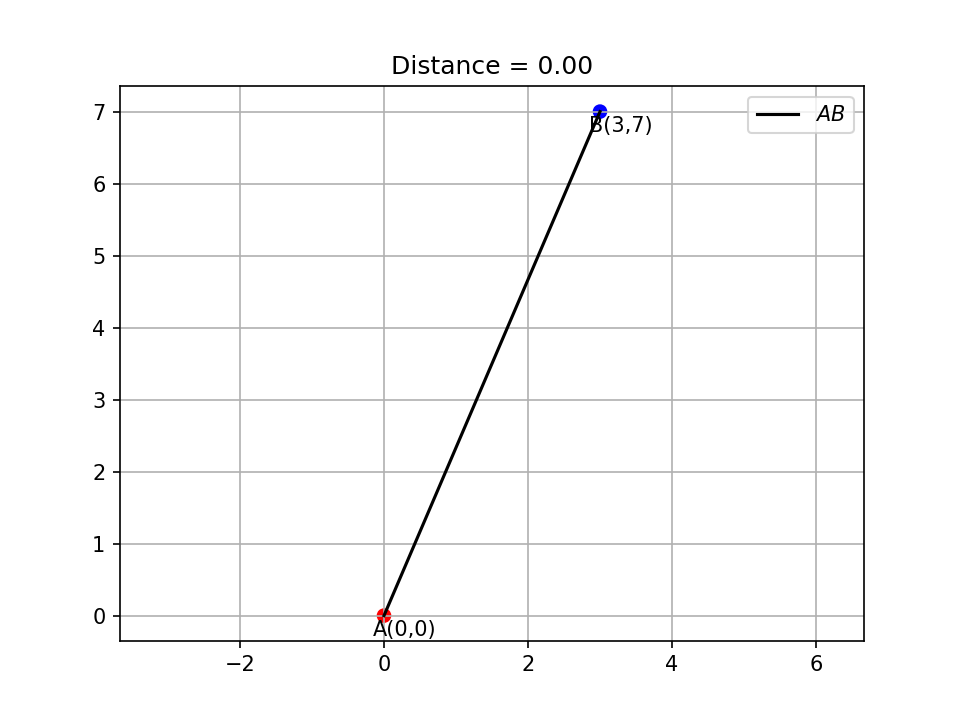
\includegraphics[width=0.75\columnwidth]{figs/2.png}
\caption{\centering plot}
\label{fig:placeholder_125}
\end{figure}
\end{document}
